\documentclass[11pt]{article}
\usepackage{amsmath}
\usepackage{amssymb}
\usepackage{graphicx}
\usepackage{hyperref}
\usepackage[dvipsnames]{xcolor}

\usepackage[simplified,school]{pgf-umlcd}
\renewcommand{\umltextcolor}{black}
\renewcommand{\umlfillcolor}{SkyBlue}
\renewcommand{\umldrawcolor}{OrangeRed}

\textwidth=6.5in
\textheight=9in
\hoffset=-.75in
\voffset=-1.in
\parskip=10pt
\parindent=0pt

\usepackage{lipsum}

\begin{document}

\title{FEMgine Developers' Guide}
\author{Davide Papapicco}

\maketitle

FEMgine is an open-source project entirely written in C++ which provides the capability of discretising and solving space-time Partial Differential Equations (PDEs) using the Finite Element Method (FEM). The library is shipped as a standalone, cross-platform software package under the GNU General Public License. At this stage (date reported below the title for reference) this library is still in early pre-alpha status and development is expected to be slow but steady. As such I created this present document as a short, informal and easy-to-read guide for developers wanting to contribute to the development of the codebase. 
\newline
\newline
\noindent
\textbf{What is the main goal and scope of this project?} To create an open-source, simplified and user-friendly tool for computational scientists that are not familiar with inner workings of numerical analysis and need a quick software to simulate and validate their models using the FEM. The project was born as part of an investigation in Computational Electromagnetics (CEM) carried among the research lines of Prof. Guido Lombardi at Politecnico di Torino. To that end FEMgine has the ultimate goal of implementing Nedelec curl and div-conforming finite elements for the arbitrary-order approximation of singular vector fields.
\newline
\newline
\noindent
\textbf{Why should I care/contribute?} The philosophy at the core of FEMgine shall also be its strength, that is simplicity and fast learning for non computationally-savvy scientists thereby providing a bridge between high-performance scientific computing and casual users of software of numerical mathematics. 
\newline
\newline
\noindent
\textbf{Is another FEM open-source library really necessary?} Absolutely not. In fact we direct the reader to large, well-established collaborative projects s.a. deal.II \cite{deal.II}, FEniCSx \cite{Fenics1,Fenics2,Fenics3,Fenics4,Fenics5,Fenics6,Fenics7,Fenics8,Fenics9,Fenics10,Fenics11,Fenics12}, FreeFEM \cite{FreeFEM}, Hermes \cite{Hermes}, MFEM \cite{MFEM}, MOOSE \cite{MOOSE}, Elmer \cite{Elmer}, FEMPAR \cite{FEMPAR} and Gridap \cite{Gridap} to name but only the more famous in the international community. As mentioned before however, FEMgine puts a larger emphasis on the ease of use on the user side, by which I mean an academic of non-professional programmer that only has a minimal understanding of numerical simulations and/or computer programming.
\newline
\newline
\noindent
\textbf{Is there any convention about this guide?} Yes there is; this guide uses a conventional colour code for highlighting and distinguishing parts of the software from the rest of the text. Specifically \colorbox{lightgray}{these} boxes either indicate a file, directory or third-party software program (not necessarily integrated or used by FEMgine) while \colorbox{cyan}{these} boxes refer to FEMgine's own classes, attributes, methods etc... Finally \colorbox{lime}{these} boxes are used to show terminal commands or specific code snippets/syntax.

\tableofcontents

\section{Library structure}
\noindent
Upon downloading the root folder of the software presents the following directories:
\begin{itemize}
    \item \colorbox{lightgray}{src}: contains the core classes and algorithms for the implementation of the FEM;
    \item \colorbox{lightgray}{utilities}: series of tools for support of the functioning and interface of the library;
    \item \colorbox{lightgray}{tutorials}: test cases showing the usage of the software for different applications.
\end{itemize}

\subsection{Third-party dependencies}
FEMgine is standalone and open-source and thus it relies on very few third-party libraries in order to accomplish its goals, namely:
\begin{itemize}
    \item \colorbox{lightgray}{Eigen}: for high-performance matrix and linear algebra data-structures and algorithms;
    \item \colorbox{lightgray}{OpenGL}: for post-processing and results visualisation purposes.
\end{itemize}

\subsection{Building the library}
The standard usage of this package is to create applications that are linked to the static library \colorbox{lightgray}{libfemgine}; this is build from source using \colorbox{lightgray}{CMake} to ensure portability across multiple OSs and CPU architectures.

\section{Code guide}
\noindent
The software is written in object-oriented paradigm and each of the classes that have been implemented accomplish a unique and specific goal within the library. The general implementation philosophy throughout the library's source code is that class declaration and definition are kept separate with the former always written in an header file (\colorbox{lightgray}{.h} extension) carrying the same name of the class that it declares, while the latter is always present in a source file (\colorbox{lightgray}{.cpp} extension) providing all the definitions of the class' methods.

\subsection{Fundamental classes}
The library is composed of several classes that are all derived from two base/parent classes, namely the \colorbox{cyan}{Entity} and \colorbox{cyan}{Mesh} classes. A third fundamental class is the \colorbox{cyan}{EntityList} class although it is not inherited by any other derived class in the library.

\subsubsection{The \colorbox{cyan}{Entity} class}
This class is the abstraction of every structure in the codebase that is indexed within a set of similar assets. In FEM much of the heavier workload at development stage goes into the proper and efficient formatting of the data-structures and local-to-global index mapping; as such there is a need to address a diverse set of items ranging from the geometrical framework as in the \colorbox{cyan}{Point}, \colorbox{cyan}{Line} or the \colorbox{cyan}{Element} class itself to entities more to the context of numerical discretisation of PDEs s.a. \colorbox{cyan}{DOF}.

\subsubsection{The \colorbox{cyan}{EntityList} class}
In order to efficiently store, access and operate onto the objects of the various classes derived from \colorbox{cyan}{Entity} a structure similar to the \colorbox{lime}{list} in Python has been implemented. This class is particularly useful to keep track of the local-to-global index mapping of the items stored in it (as described above). Its fundamental (\colorbox{lime}{private}) attribute is a \colorbox{lime}{std::vector$<$}\colorbox{cyan}{Entity}\colorbox{lime}{$>$} container making this a highly templatised class. It features an accessor method \colorbox{lime}{get$\_$list()} making it compatible with range-based loops in C++.

\subsubsection{The \colorbox{cyan}{Mesh} class}
As in many other scientific suites, the mesh is one of the fundamental pieces of information of the model while also being one of the most crucial, large and easy to misconceive class in OOP. This class contains a vast amount of information through its \colorbox{lime}{private} and \colorbox{lime}{protected} attributes while at the same time it must store such critical information in a way that can be accessed by its child classes and transformed/processed according to the user's specific needs. Of course the vast majority of its attributes are \colorbox{cyan}{EntityList} of items s.a. the various finite elements with their degrees of freedom and geometrical information as well as linear algebra operators for the assembly and the solution of the discrete linear system of equations.

\newpage
\subsection{Inheritance diagrams}
Below there are UML-like class diagrams for the three fundamental classes.
\newline
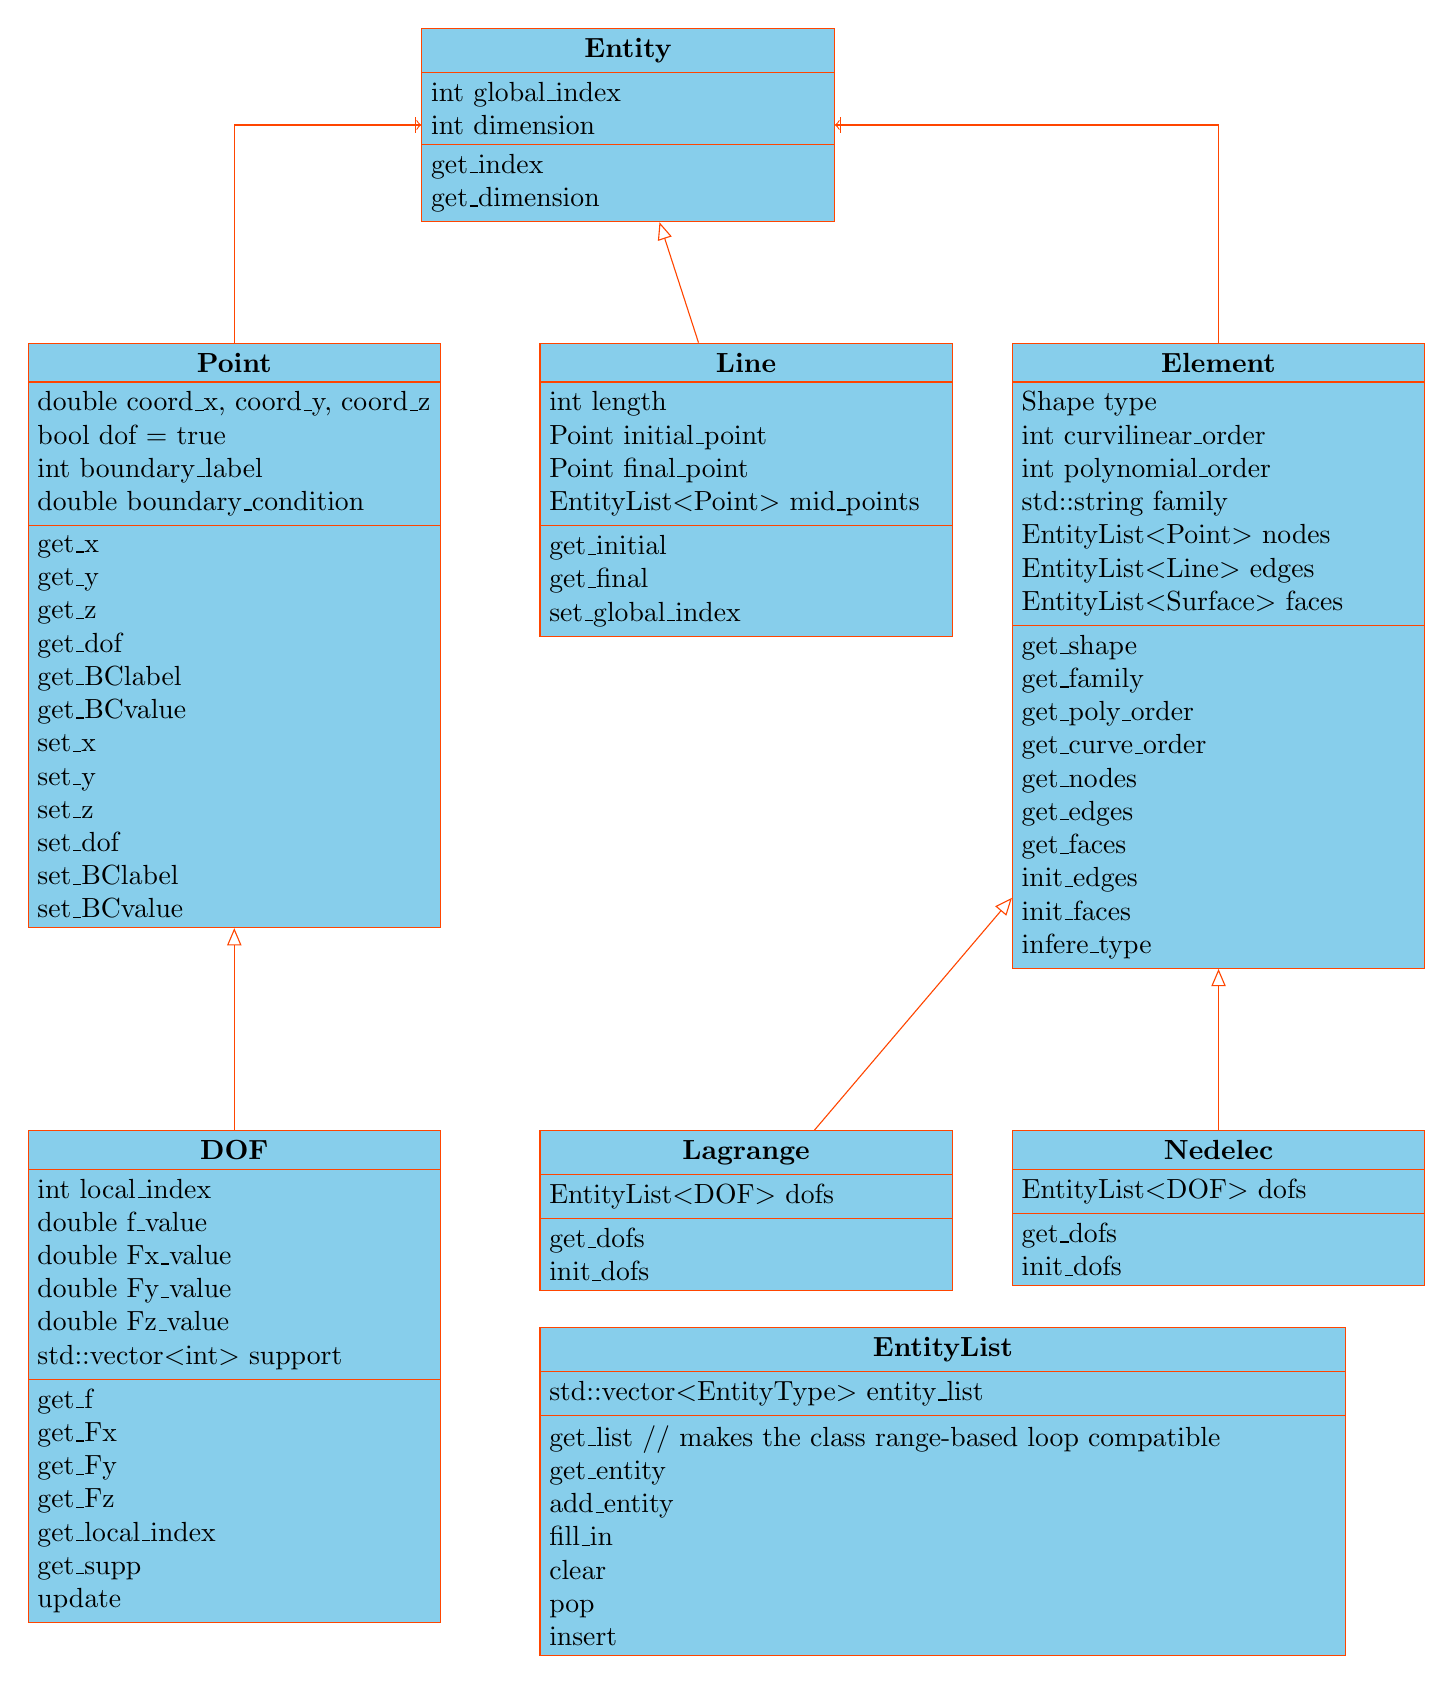
\begin{tikzpicture}
    \begin{class}[text width=5cm]{Entity}{0,0}
        \attribute{int global\_index}
        \attribute{int dimension}

        \operation{get\_index}
        \operation{get\_dimension}
    \end{class}

    \begin{class}[text width=5cm]{Point}{-5,-4}
        \attribute{double coord\_x, coord\_y, coord\_z}
        \attribute{bool dof = true}
	  \attribute{int boundary\_label}
	  \attribute{double boundary\_condition}

        \operation{get\_x}
        \operation{get\_y}
        \operation{get\_z}
        \operation{get\_dof}
        \operation{get\_BClabel}
        \operation{get\_BCvalue}
        \operation{set\_x}
        \operation{set\_y}
        \operation{set\_z}
        \operation{set\_dof}
        \operation{set\_BClabel}
        \operation{set\_BCvalue}
    \end{class}

    \draw[OrangeRed,-|>](Point)|-node[above,sloped,black]{}(Entity);

    \begin{class}[text width=5cm]{Line}{1.5,-4}
        \inherit{Entity}
        \attribute{int length}
        \attribute{Point initial\_point}
        \attribute{Point final\_point}
        \attribute{EntityList$<$Point$>$ mid\_points}

        \operation{get\_initial}
        \operation{get\_final}
        \operation{set\_global\_index}
    \end{class}

    \begin{class}[text width=5cm]{Element}{7.5,-4}
        \attribute{Shape type}
        \attribute{int curvilinear\_order}
        \attribute{int polynomial\_order}
        \attribute{std::string family}
        \attribute{EntityList$<$Point$>$ nodes}
        \attribute{EntityList$<$Line$>$ edges}
        \attribute{EntityList$<$Surface$>$ faces}

        \operation{get\_shape}
        \operation{get\_family}
        \operation{get\_poly\_order}
        \operation{get\_curve\_order}
        \operation{get\_nodes}
        \operation{get\_edges}
        \operation{get\_faces}
        \operation{init\_edges}
        \operation{init\_faces}
        \operation{infere\_type}
    \end{class}

    \draw[OrangeRed,-|>](Element)|-node[above,sloped,black]{}(Entity);

    \begin{class}[text width=5cm]{DOF}{-5,-14}
        \inherit{Point}
        \attribute{int local\_index}
        \attribute{double f\_value}
        \attribute{double Fx\_value}
        \attribute{double Fy\_value}
        \attribute{double Fz\_value}
        \attribute{std::vector$<$int$>$ support}

        \operation{get\_f}
        \operation{get\_Fx}
        \operation{get\_Fy}
        \operation{get\_Fz}
        \operation{get\_local\_index}
        \operation{get\_supp}
        \operation{update}
    \end{class}

    \begin{class}[text width=5cm]{Lagrange}{1.5,-14}
        \inherit{Element}
        \attribute{EntityList$<$DOF$>$ dofs}
        
        \operation{get\_dofs}
        \operation{init\_dofs}
    \end{class}

    \begin{class}[text width=5cm]{Nedelec}{7.5,-14}
        \inherit{Element}
        \attribute{EntityList$<$DOF$>$ dofs}
        
        \operation{get\_dofs}
        \operation{init\_dofs}
    \end{class}

    \begin{class}[text width=10cm]{EntityList}{4,-16.5}
        \attribute{std::vector$<$EntityType$>$ entity\_list}
        
        \operation{get\_list // makes the class range-based loop compatible}
        \operation{get\_entity}
        \operation{add\_entity}
        \operation{fill\_in}
        \operation{clear}
        \operation{pop}
        \operation{insert}
    \end{class}
\end{tikzpicture}

\newpage
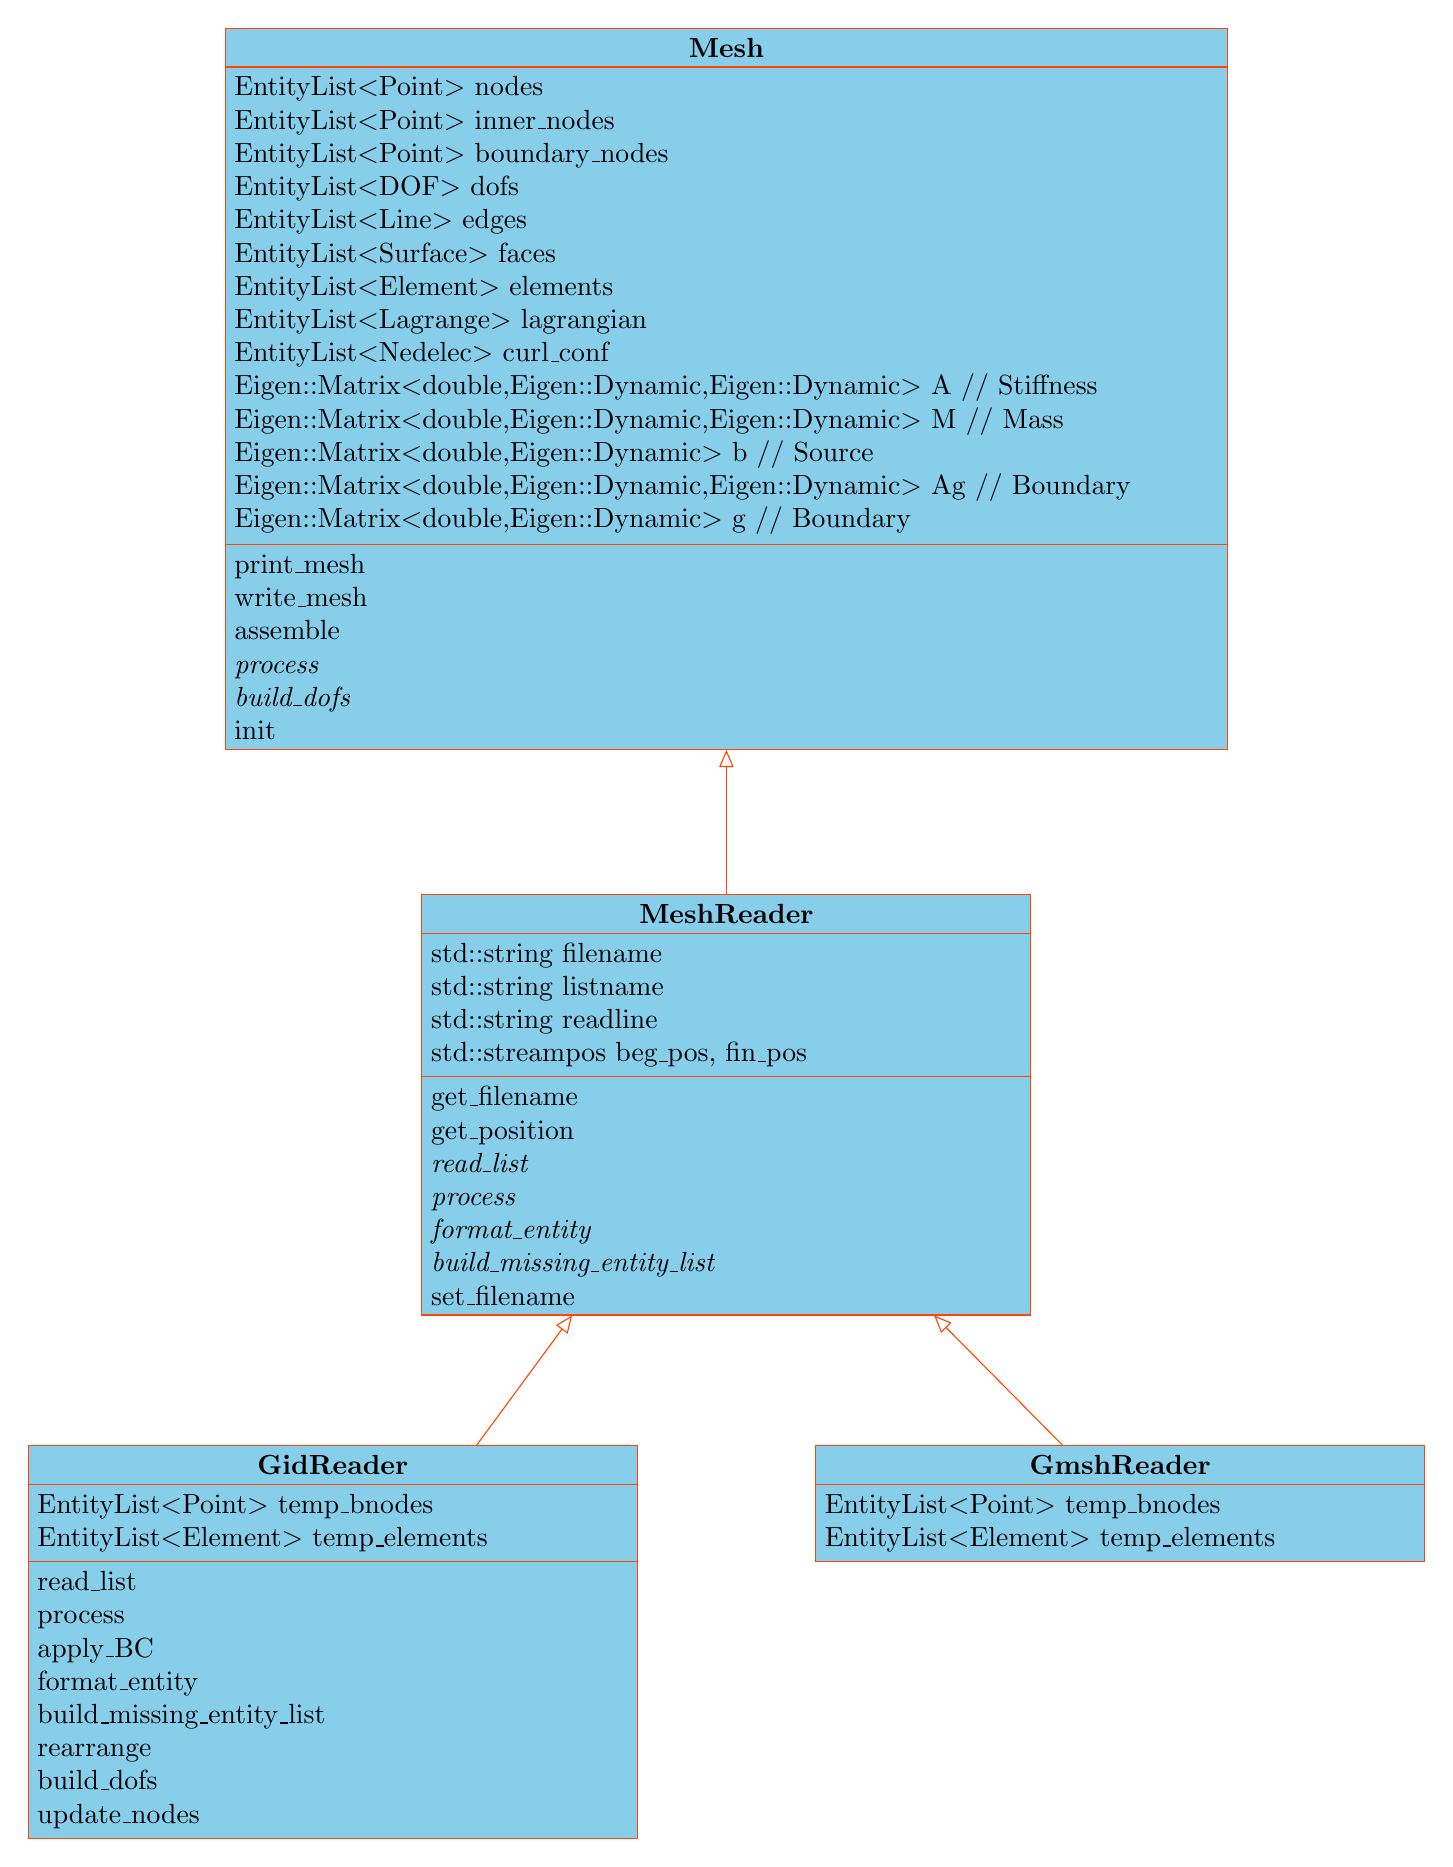
\begin{tikzpicture}
    \begin{class}[text width=12.5cm]{Mesh}{0,0}
        \attribute{EntityList$<$Point$>$ nodes}
        \attribute{EntityList$<$Point$>$ inner\_nodes}
        \attribute{EntityList$<$Point$>$ boundary\_nodes}
        \attribute{EntityList$<$DOF$>$ dofs}
        \attribute{EntityList$<$Line$>$ edges}
        \attribute{EntityList$<$Surface$>$ faces}
        \attribute{EntityList$<$Element$>$ elements}
        \attribute{EntityList$<$Lagrange$>$ lagrangian}
        \attribute{EntityList$<$Nedelec$>$ curl\_conf}
        \attribute{Eigen::Matrix$<$double,Eigen::Dynamic,Eigen::Dynamic$>$ A // Stiffness}
        \attribute{Eigen::Matrix$<$double,Eigen::Dynamic,Eigen::Dynamic$>$ M // Mass}
        \attribute{Eigen::Matrix$<$double,Eigen::Dynamic$>$ b // Source}
        \attribute{Eigen::Matrix$<$double,Eigen::Dynamic,Eigen::Dynamic$>$ Ag // Boundary}
        \attribute{Eigen::Matrix$<$double,Eigen::Dynamic$>$ g // Boundary}

        \operation{print\_mesh}
        \operation{write\_mesh}
        \operation{assemble}
        \operation[0]{process}
        \operation[0]{build\_dofs}
        \operation{init}
    \end{class}

    \begin{class}[text width=7.5cm]{MeshReader}{0,-11}
        \inherit{Mesh}
        \attribute{std::string filename}
        \attribute{std::string listname}
        \attribute{std::string readline}
        \attribute{std::streampos beg\_pos, fin\_pos}
        
        \operation{get\_filename}
        \operation{get\_position}
        \operation[0]{read\_list}
        \operation[0]{process}
        \operation[0]{format\_entity}
        \operation[0]{build\_missing\_entity\_list}
        \operation{set\_filename}
    \end{class}

    \begin{class}[text width=7.5cm]{GidReader}{-5,-18}
        \inherit{MeshReader}
        \attribute{EntityList$<$Point$>$ temp\_bnodes}
        \attribute{EntityList$<$Element$>$ temp\_elements}
        
        \operation{read\_list}
        \operation{process}
        \operation{apply\_BC}
        \operation{format\_entity}
        \operation{build\_missing\_entity\_list}
        \operation{rearrange}
        \operation{build\_dofs}
        \operation{update\_nodes}
    \end{class}
    
    \begin{class}[text width=7.5cm]{GmshReader}{5,-18}
        \inherit{MeshReader}
        \attribute{EntityList$<$Point$>$ temp\_bnodes}
        \attribute{EntityList$<$Element$>$ temp\_elements}
    \end{class}
\end{tikzpicture}

\section{Meshing}
\noindent
At the present moment FEMgine does not feature its own meshing utility and instead it relies on ad-hoc external software to export the data-structure and appropriately interface with.

\subsection{\colorbox{lightgray}{GiD}}
The \colorbox{lightgray}{GiD} interface is implemented through the \colorbox{cyan}{GidReader} derived class. This class is responsible for a lot of heavy-lifting in the pre-processing of the raw mesh input file as it extracts and formats all the existing information provided by \colorbox{lightgray}{Gid}, namely the discrete nodes \colorbox{lime}{Coordinates}, the vertices of the \colorbox{lime}{Elements} and the labels and indices of the \colorbox{lime}{Boundary Nodes}. \color{red} \textbf{ATTENTION:} \color{black}: in \colorbox{lightgray}{GiD}'s ouput raw mesh \colorbox{lightgray}{.txt} file these last entities are encoded under the target \colorbox{lime}{Mesh Entities}; the user must rename the beginning and end target as specified. It also initialises all the relevant \colorbox{cyan}{Entity} and \colorbox{cyan}{EntityList} with appropriate information and, where necessary, it computes the missing ones s.a. the list of \colorbox{cyan}{Line} and \colorbox{cyan}{Surface} delimiting the elemental domain (see the \colorbox{lime}{build$\_$missing$\_$entity$\_$list()} and \colorbox{lime}{build$\_$dofs()} private methods).

\subsection{\colorbox{lightgray}{gmsh}}
The \colorbox{lightgray}{gmsh} interface has not yet been implemented.

\section{Pre-processing}
\noindent
As discussed above, FEMgine relies on external meshing software to provide the initial raw mesh data. This necessarily entails that manipulation and extraction of further information from the raw data has to be performed for a functioning application. Each mesh interface class (e.g. \colorbox{cyan}{GidReader}) implements different type of pre-processing of such data, as different outputs will be provided by the various mesh utilities.

\subsection{Numbering conventions}
One fundamental aspect for FEMgine is to adopt a unique, efficient and consistent notation for numbering the various \colorbox{cyan}{Entity} in the mesh. For the local numbering of the elements' vertices, edges and faces we refer to the \colorbox{lightgray}{doc/numbering$\_$conventions} subdirectory containing illustrations of the adopted convention, heavily inspired by \cite{TAP97} (especially for the Nedelec curl-conforming finite elements \cite{Nedelec}).

\subsection{Boundary conditions}
At the moment FEMgine only supports the imposition of Dirichlet boundary conditions. The boundary function $g_D(\mathbf{x}),\;\forall\Gamma\in\partial\Omega$ is defined by the user and passed through the \colorbox{cyan}{MeshReader} interface to the library. Each edge $\Gamma$ of the polygonal boundary $\partial\Omega$ is identified in the meshing facility (e.g. \colorbox{lightgray}{GiD}) by a unique numerical label. The user thus associates (in FEMgine) the desired boundary function to a particular label and the \colorbox{lime}{apply$\_$BC} method assigns the computed value to every node in the mesh labelled appropriately.

\section{Finite elements}
\noindent
Although the \colorbox{cyan}{Element} class derives from the \colorbox{cyan}{Entity} class, it acts as base class for the various types of finite elements to be implemented (according to Ciarlet's definition \cite{Ciarlet}). The fundamental attributes are of course \colorbox{cyan}{EntityList} encoding the geometrical information of the element however it also stores the order of approximation. \color{red} \textbf{ATTENTION:} \color{black}: it must be noted that the \colorbox{cyan}{DOF} list is not a member attribute as this class does not initialise a specific type of finite element. These \colorbox{cyan}{EntityList} is instead initialised by the derived classes associated to the different types of finite element (any finite element has its own type of degree of freedom). Another fundamental member attribute of this parent class is the \colorbox{cyan}{Shape} associated to the geometry of the finite element. The \colorbox{cyan}{Shape} class stores all the information relevant to the mapping between the physical element to the reference element (thus involving its Jacobian) s.a. orientation of the faces for $3$D elements, the area and volume etc...

\subsection{The \colorbox{cyan}{Lagrange} element}
In the Lagrangian finite elements the degrees of freedom are \colorbox{cyan}{DOF} the values that the unknown numerical solution at specified points within the elemental domain (either on its boundary or within them). This class has features a parametric copy-constructor 
\newline
\noindent
\colorbox{lime}{Lagrange(Element $\&$copy$\_$element, EntityList$<$Point$>$ arg$\_$nodes, std::string* arg$\_$family, int* arg$\_$order)} that automatically initialises the correct \colorbox{cyan}{EntityList$<$DOF$>$} based on the parent object geometrical attributes and the passed-by-reference user information regarding the polynomial order of the approximation subspace.

\subsection{The \colorbox{cyan}{Nedelec} element}
This type of finite element is yet to be implemented.

\section{Discrete linear system}
\noindent
The discretised linear system assembled by FEMgine has the form $\mathbf{A}\mathbf{u}_h=\mathbf{b}-\mathbf{A}_g\mathbf{g}_D$ where $\mathbf{A}$ is the stiffness matrix associated to the discretisation of the differential operator/bilinear form in the weak formulation, $\mathbf{b}$ is the source vector collecting the values of the forcing (known) function $f(\mathbf{x})$ and $\mathbf{A}_g, \mathbf{g}_D$ are the boundary matrix and vector (respectively) collecting the information at the boundary for the model. The \colorbox{lime}{RHS} is encoded in FEMgine by the (algebric, element-wise) sum of the source vector and the product $\mathbf{A}_g\mathbf{g}_D$.

\subsection{Assembly}
The discretisation of the bilinear form is carried by the \colorbox{lime}{assemble} member function of the \colorbox{cyan}{Mesh} class as it is independent on the interface with meshing utility.

\subsection{Solution}
The solution of the linear system is performed using \colorbox{lightgray}{Eigen} built-in solvers and depending on the structure and denseness of the \colorbox{lime}{RHS}.

\section{Post-processing}
\noindent
The post-processing of the numerical results is not yet implemented however it shall provide error-estimation capabilities (both a-priori and a-posteriori), mesh and subspace local refinement and results visualisation.

\subsection{Visualisation}
The graphical visualisation of the numerical solution and its (discretised) mesh domain is yet to be implemented however it shall be performed in \colorbox{lightgray}{OpenGL}.

\newpage
\bibliographystyle{elsarticle-num}
\bibliography{refs.bib}

\end{document}